\documentclass[a4paper]{jpconf}
% \usepackage[square,sort&compress,sectionbib]{natbib}

\usepackage{amsmath}
\usepackage{graphicx}
\usepackage{wrapfig}
\usepackage[table,xcdraw]{xcolor}



% define color
\definecolor{olivegreen}{RGB}{34,139,34}
\definecolor{darkorange}{RGB}{255,140,0}

\begin{document}
\title{Preliminary indirect measurement of cosmic-ray proton spectrum using Earth's $\gamma$-ray data from {\it Fermi} Large Area Telescope}

\author{Patomporn Payoungkhamdee}
\address{Department of Physics, Faculty of Science, Mahidol University}
% \address{Production Editor, \jpcs, \iopp, Dirac House, Temple Back, Bristol BS1~6BE, UK}

\ead{patomporn.pay@gmail.com}

\begin{abstract}
Cosmic rays (CRs) are high-energy particles, mostly protons, propagating in space. The rigidity (momentum per charge) spectrum of CRs is well described by a power law for which the spectral index is approximately 2.8 around 30 - 1000 GV. Recent measurements by PAMELA and AMS-02 indicate an abrupt change of the CR proton spectral index at about 340 GV. When CRs interact with the Earth's upper atmosphere, $\gamma$ rays can be produced and detected by space-based detectors. Here we use the Earth's $\gamma$-ray data collected by the {\it Fermi} Large Area Telescope along with a proton-air interaction model to indirectly determine the CR proton spectral index and compare against observations by other instruments.
\end{abstract}

\section{Introduction}
Cosmic-ray are high energy particle which mainly come from the outer space which can penetrate and interact with the Earth's atmosphere \cite{HESS,Pacini,Clay}.
The shark peak of gamma-ray emission from Earth's limb are mainly come from the interaction of CRs with the atmospheric molecules \cite{Warit2009}.

There are many possible phenomena of acceleration mechanism in the
space that could produce high energy particles. The characteristic of acceleration mechanism could roughly be distinguished by a spectral index in the arrival of cosmic rays spectrum in rigidity.
The breaking point of the spectrum mainly come from the overlapped region of acceleration mechanism that could be an evidence to explore a new candidate of cosmic ray source.

In 2011, PAMELA detector indicated that there is a breakpoint of cosmic-ray protons spectrum around 240 GV \cite{PAMELA}.
Furthermore, AMS-02 also found a drastic change of cosmic-ray proton spectrum at around 336 GV \cite{AMS-02}.
From the previous work, 5 years of \textit{Fermi} Large Area Telescope
(\textit{Fermi}-LAT) observation data has been analyzed to trace back
the characteristic of CR proton spectrum where the result imply that there is
a breaking of spectral indice around 200 GeV where the statistical significance
is around 2$\sigma$ \cite{previouswork}. In this work, 9 years of \textit{Fermi}-LAT
data would be use for finding the spectral indices of CR proton between energy
hundred MeV to a TeV range.

\section{Methodology}
\subsection{Data selection and $\gamma$-ray flux extraction}

We use $\sim9$ years (7 Aug 2008 - 16 Oct 2017) of the latest version
(P8R2 ULTRACLEANVETO V6) of the LAT's photon data between 10 GeV to 1 TeV.
We observe $\gamma$ rays from the Earth's thin upper atmosphere by selecting the
nadir angle ($\theta_{\rm NADIR}$) from $68.4^\circ$ to $70.0^\circ$ \cite{previouswork} as
demonstrated in Figure~\ref{gamma_production_schematic}. The incidence angle cut,
$\theta_{\rm LAT}<70^\circ$, is also applied.


% \begin{figure}[h!]
%     \centering
%     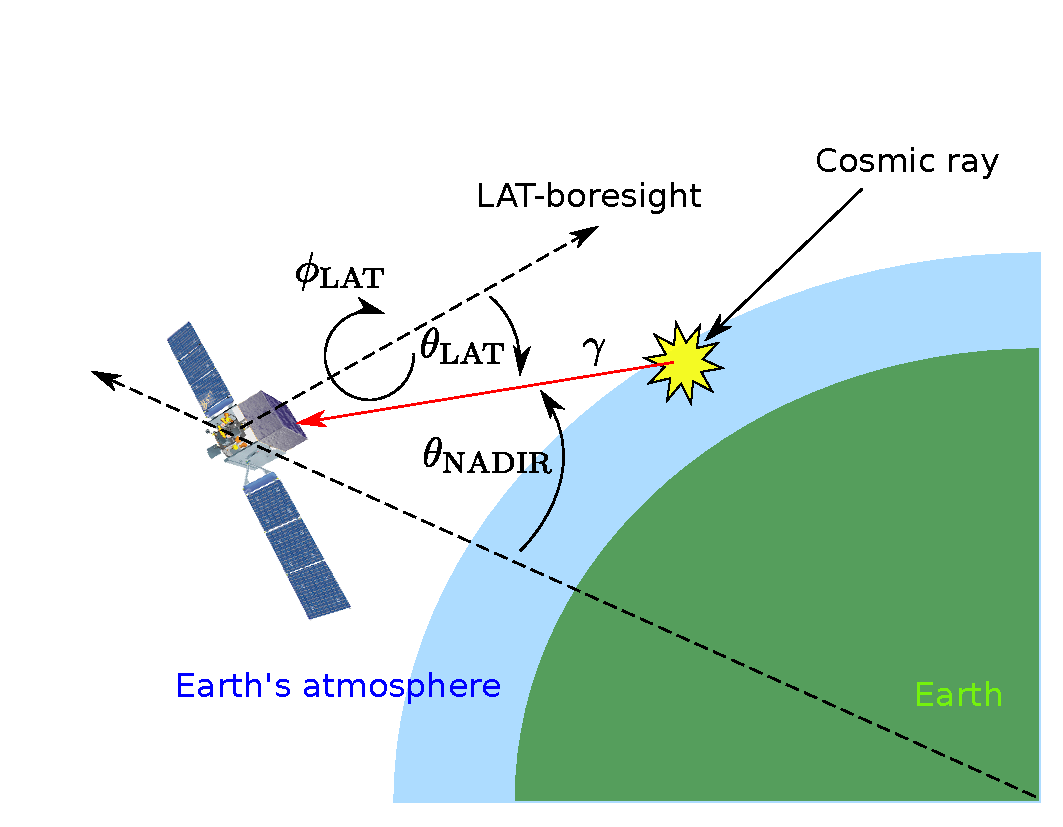
\includegraphics[width=0.5\textwidth]{img/gamma_production_schematic}
%     \caption{Schematic of $\gamma$-ray production}
%     \label{gamma_production_schematic}
% \end{figure}

% \begin{wrapfigure}{r}{0.5\textwidth}
%     \begin{center}
%         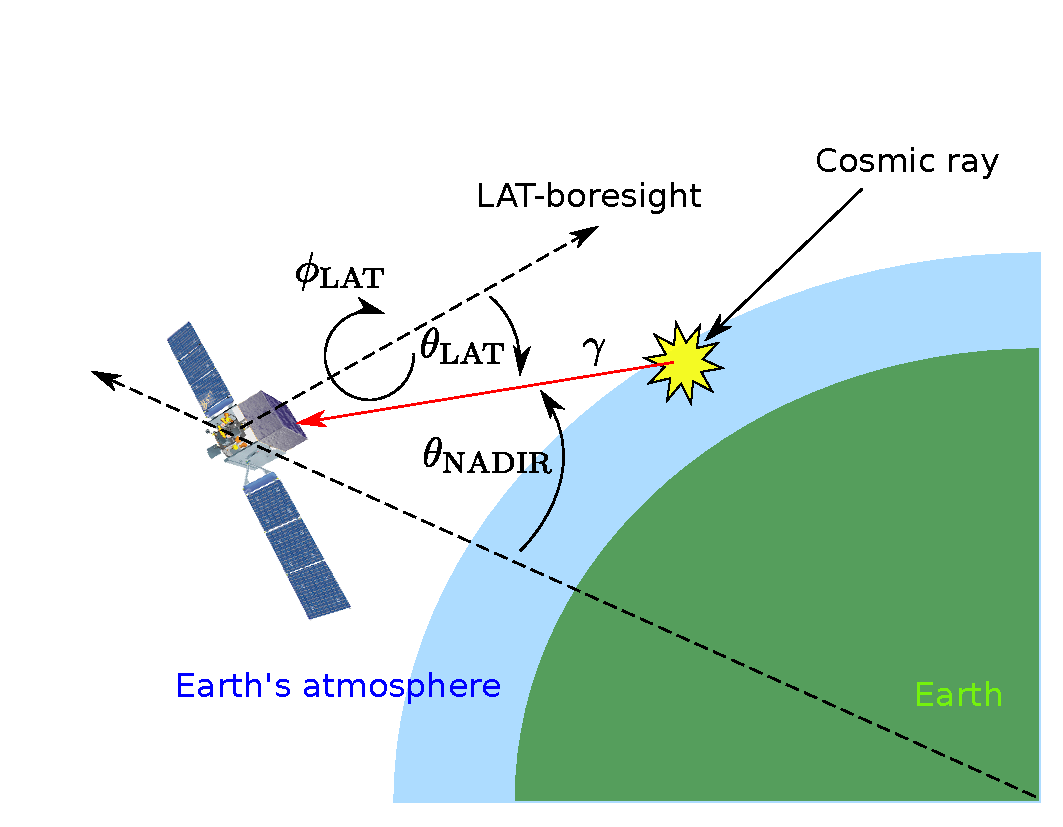
\includegraphics[width=0.5\textwidth]{img/gamma_production_schematic}
%     \end{center}
%     \caption{Schematic of $\gamma$-ray production}
%     \label{gamma_production_schematic}
% \end{wrapfigure}

\begin{figure}[h]
    \begin{minipage}{0.45\textwidth}
        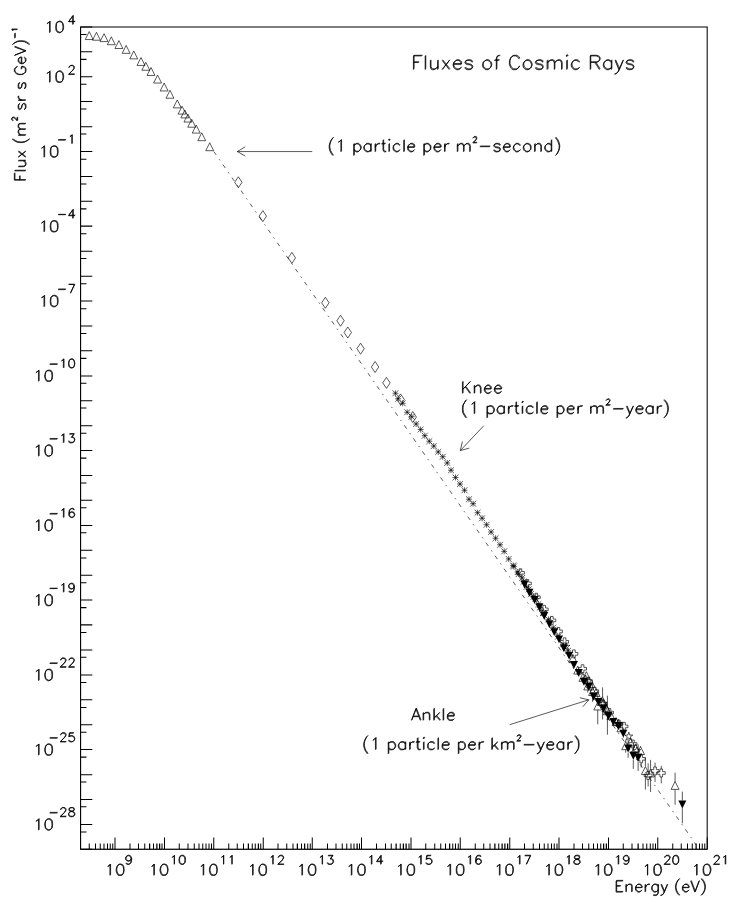
\includegraphics[width=\textwidth]{img/cr_knee_ankle}
        \caption{All-particle CR spectrum taken from \cite{Swordy2001}.}
        % \caption{The all particle spectrum of cosmic rays, image taken from }
        \label{cr_knee_ankle}
    \end{minipage}\hspace{2pc}
    \begin{minipage}{0.55\textwidth}
        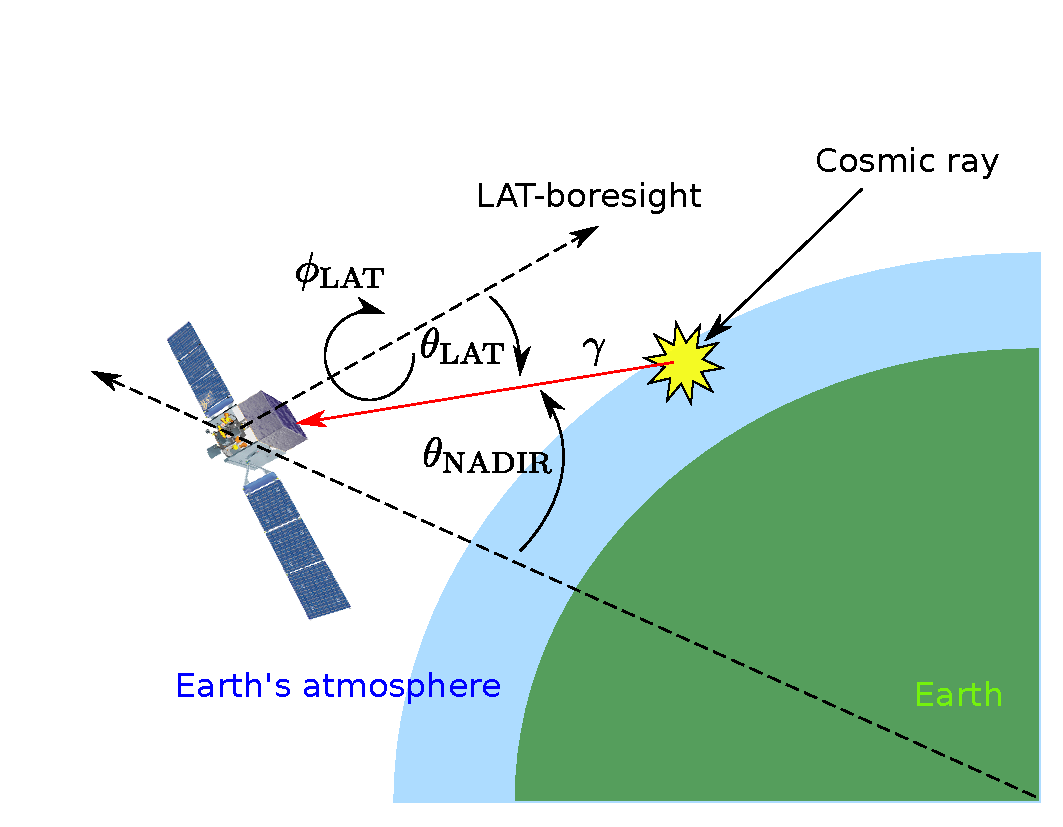
\includegraphics[width=\textwidth]{img/gamma_production_schematic}
        \caption{Schematic of high-energy Earth's $\gamma$-ray production}
        \label{gamma_production_schematic}
    \end{minipage} 
\end{figure}

% The observed flux is defined as differential flux where the governing equation
% for the calculation is represented as equation (\ref{flux_definition})
The observed flux for a given energy bin is calculated using
\begin{equation}
    \textbf{Flux} \equiv \frac{dN_\gamma}{dE} = \frac{\int_{\textrm{Limb region}}(\textrm{Count map}/\textrm{Exposure map})}{\Delta\Omega\Delta E }
    .\label{flux_definition}
\end{equation}

% Where count map is filled up with selected $\gamma$-ray and 
Here the count map is filled with numbers of photons, the exposure map represents 
the exposure time as well as the effective area of spacecraft 
which is a function of energy and $\theta_{\rm LAT}$, $\Delta E$ is the energy bin width,
and $\Delta\Omega$ is the solid angle of the thin-target Earth's limb region.
% Procedure of computation is begin with the requirement of 25 bins of histogram of
% the $\gamma$-ray flux which contain a various median of energy in each bin.
We perform the analysis with 25 bins of energy, equally spaced in logarithmic scale.
% Consequently, the number of count map and exposure map will be exactly the same as
% the energy bins. The calculation of exposure map is done by using log file of the
% spacecraft combine with the responsiveness of the spacecraft which has to be consider
% in every step time while spacecraft is online. 
For a given energy bin, the exposure map is calculated using the spacecraft's position
and orientation recorded in 30-second time steps, each of which involves a complex
coordinate transformation to create a map in the zenith-azimuth system.
Such computationally intensive task requires parallel
processing with Master-Slave technique that we have developed.
% which cause a huge amount of computing process.
% That is the reason why paralleling processing with Master-Slave technique is
% applied in this work.


\subsection{Interaction model}
In this work, we test 2 models of CR protons: single-power law (SPL) model
containing one spectral index, and broken-power law (SPL) model containing two
spectral indices with a break energy.

% The model for a scattering amplitude from hadronic collision \cite{K&Omodel}
% that could produce a photon as a secondary product which could be
% detected by \textit{Fermi}-LAT as equation \ref{eq:interaction_model}.
According to \cite{K&Omodel}, the secondary photon spectrum from proton-proton
collisions could be summarized by

\begin{equation}
    \frac{dN_\gamma}{dE_\gamma}\propto \int^{E_{\text{max}}}_{E_\gamma} dE'\frac{dN_p}{dE'} \frac{d\sigma^{pp\rightarrow\gamma}(E',E_\gamma)}{dE_\gamma}
    ,\label{eq:interaction_model}
\end{equation}

where here $dN_\gamma/dE_\gamma$ is the measured Earth's limb $\gamma$-ray spectrum,
$dN_p/dE'$ is the CR proton model, and $\sigma^{pp\rightarrow\gamma}$ is the interaction
cross section.
We take into account the contribution from CR He particles to the production of secondary
photons by using the cross section ratio ($\sigma_{\rm HeN}/\sigma_{p\rm N}$) from
\cite{WAtwater} and the He spectrum measurement by \cite{AMS-02Helium}. This modifies
Eq.~(\ref{eq:interaction_model}) to
% For the real use case, the interaction of an alphaparticle with the air
% has a significant contribution to the secondary photon.
% A modification of He-air interaction could be
% applied by using a fraction of cross-section from a given atomic number
% \cite{WAtwater}. The helium spectrum in rigidity is taken from the real
% measurement \cite{AMS-02Helium}. Then the input of the modified model
% is left only a proton spectrum.

\begin{equation}
    \frac{dN_{\gamma}}{dE_\gamma}(E_\gamma) \propto
    \sum_{E'_i}\left[\frac{E'_i}{E_{\gamma}}\Delta(\ln E'_i) \right]
    \left[ 
        f_{pp}\frac{dN_p}{dE'_i}
        \left\{
            1+\frac{\sigma_{\text{HeN}}}{\sigma{p\rm N}}\left(\frac{dN_p}{dR}\right)^{-1} \frac{dN_{\text{He}}}{dR} \frac{dR_{\text{He}}}{dR_p} 
        \right\}
    \right]
    ,\label{eq:derived_model}
\end{equation}

where $f_{pp} \equiv E_\gamma(d\sigma^{ij\rightarrow\gamma}/dE_\gamma)$
is the interaction cross section table in \cite{K&Omodel}.

\subsection{Optimization}

We use the SPL and BPL models for $dN_p/dE'$ in Eq.~(\ref{eq:derived_model}) and vary their parameters
(normalization, spectral indices, break energy) so that the resulting $dN_\gamma/dE_\gamma$
from the model fits to the measured Earth's limb $\gamma$-ray spectrum with maximum
likelihood. We employ the particle swarm optimization (PSO) \cite{pso_optimize} as our fitting algorithm
because PSO is efficient at avoiding local maxima and reaching the global maximum in
this multi-parameter problem.
% Optimizing a problem with multiple parameters might cause a local minimum
% which will cause an early stopping of the optimization proces before 
% reaching to the global minimum. In this work, a simple gradient optimization
% with a set of different initial values yield a various output which implicitly
% imply that there are local minimum exists in this problem. 
% To get rid of the local minimum, particle swarm optimization (PSO) is applied
% to find the best fit parameters \cite{pso_optimize}.





\section{Preliminary Results}
The optimized parameters  for the SPL and BPL models are summarized in Table~\ref{tb:bestparams}. 
The best-fit $\gamma$-ray spectra from the two models
compared to the thin-target Earth's limb measurement by the LAT are illustrated
in figure~\ref{fig:gamma-flux}, showing very similar results for both models.
Since the proton-to-$\gamma$ energy conversion factor is roughly 0.17 for broad
and smooth spectra [10], our inferred CR proton spectra are valid between 60 - 2000 GV
in rigidity
% because the lower bound is a minimum rigidity of incoming proton that could produce a 10 GeV of $\gamma$-ray
% as shown in comparison with measurements by other instruments in Figure~\ref{fig:proton-flux}.
% Note that the normalizations of our work in Figure~\ref{fig:proton-flux} are scaled
% by fitting to AMS-02 data between 100~-~2000~GV.
because the lower bound is the mean rigidity of the incoming protons that produce 10-GeV $\gamma$ rays.
Our results are shown in comparison with measurements by other instruments in figure~\ref{fig:proton-flux}.
Note that the normalizations of our work in figure~\ref{fig:proton-flux} are scaled
by fitting to AMS-02 data between 100~-~2000~GV.

% eye to approximately match PAMELA data.
% has shown in Table~\ref{tb:bestparams}.
% According to figure \ref{fig:gamma-flux}, secondary $\gamma$-ray product
% from both SPL and BPL model yield a similar product via hadronic collision
% in the atmosphere. In order to validate the indirect measurement of CR proton,
% comparing with a real observations is mandatory which has shown
% in figure \ref{fig:proton-flux}. The normalization of this work is
% fitted PAMELA data to roughly scale the incident proton spectrum.

\begin{figure}[h!]
    \centering
    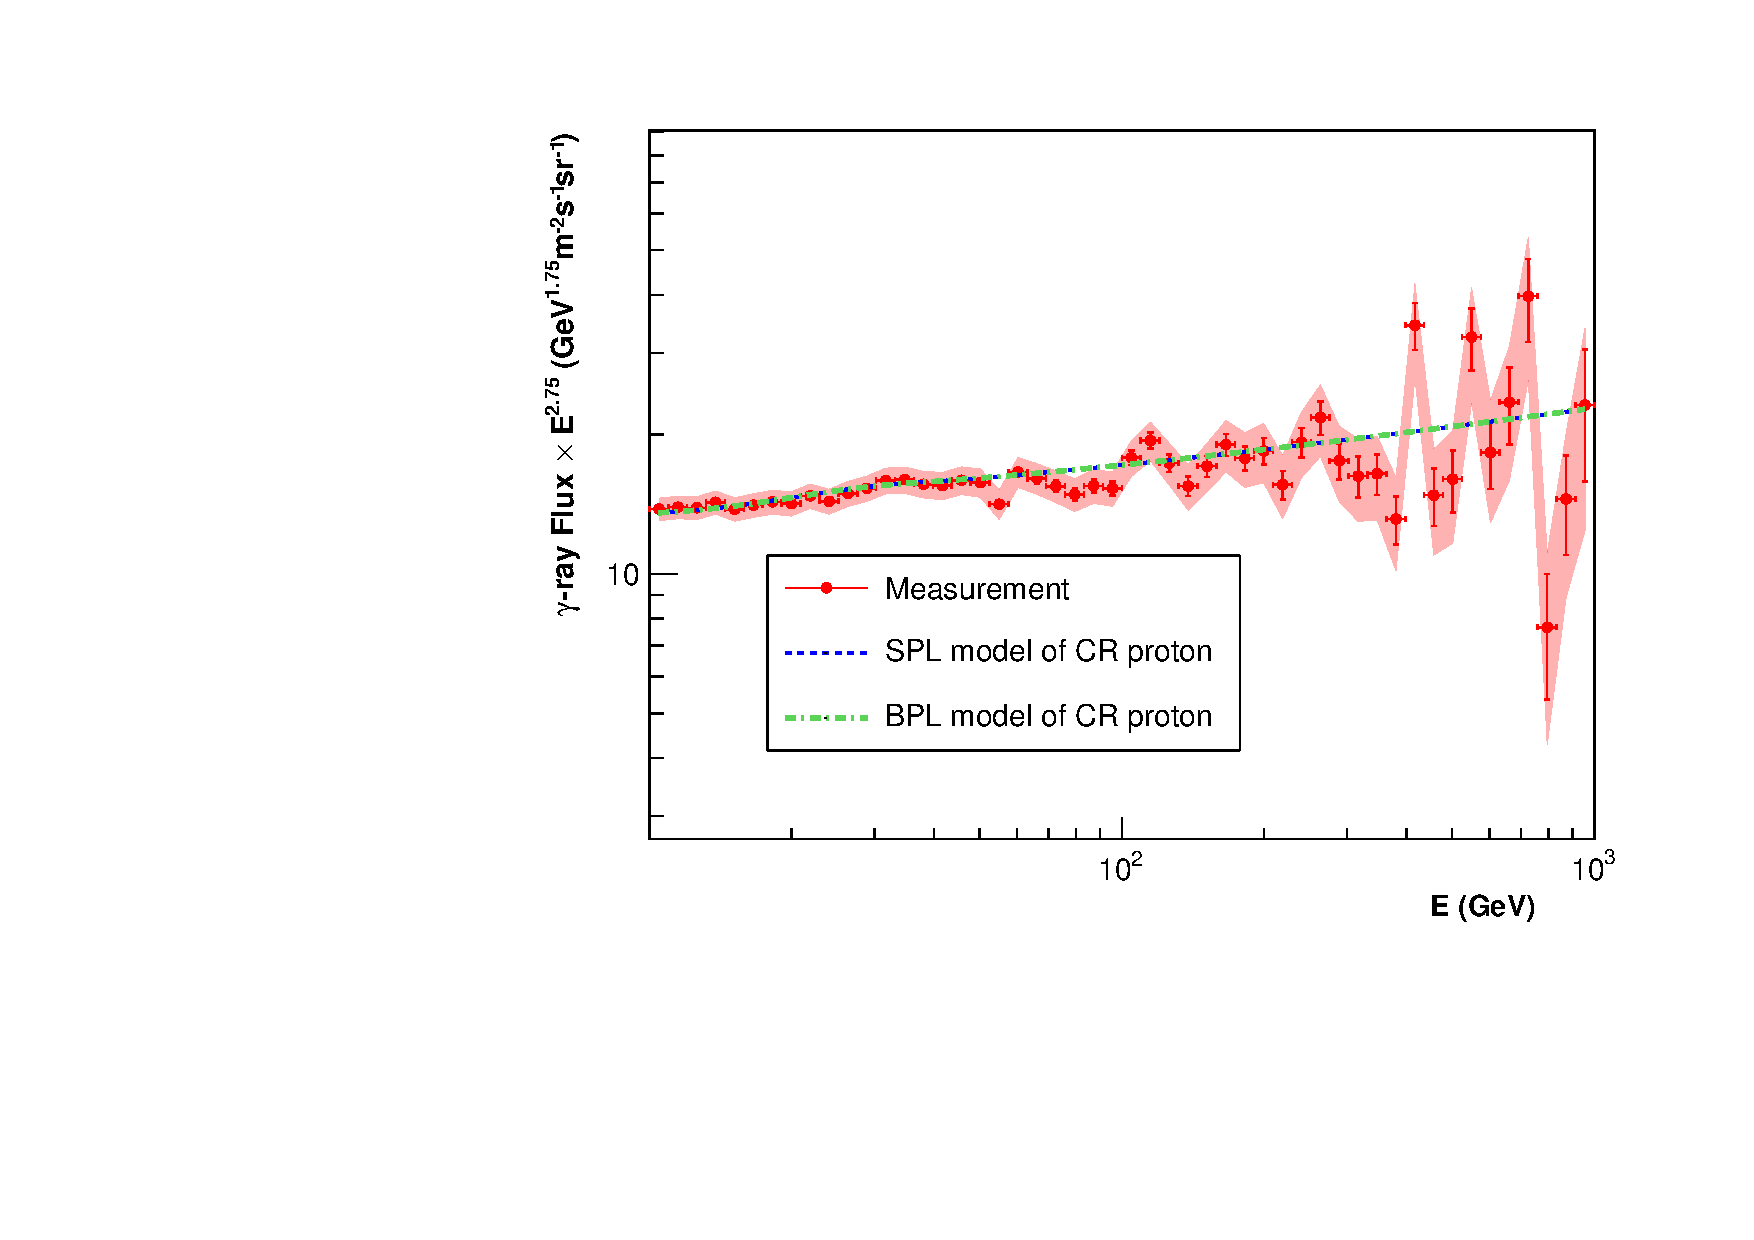
\includegraphics[width=0.7\textwidth]{img/fitted_result}
    % \caption{Measured $\gamma$-ray flux and the product from incident CRs}
    \caption{
        The $\gamma$-ray spectra calculated from the SPL (blue)
        and BPL (green) models of CR proton which best fit with the measured Earth's
        $\gamma$-ray spectrum in the thin-target regime (red).
    }
    \label{fig:gamma-flux}
\end{figure}



\begin{center}
\begin{table}[h]
\centering
\caption{Best-fit CR proton spectral parameters} 
\label{tb:bestparams}
\begin{tabular}{@{}l*{15}{l}}
\br
CR proton model&Index 1&Index 2&$E_\text{break}$ (GeV)\\
\mr
SPL&2.70&-&-\\
BPL&2.86&2.63&333\\
\br
\end{tabular}
\end{table}
\end{center}


\begin{figure}[h!]
    \centering
    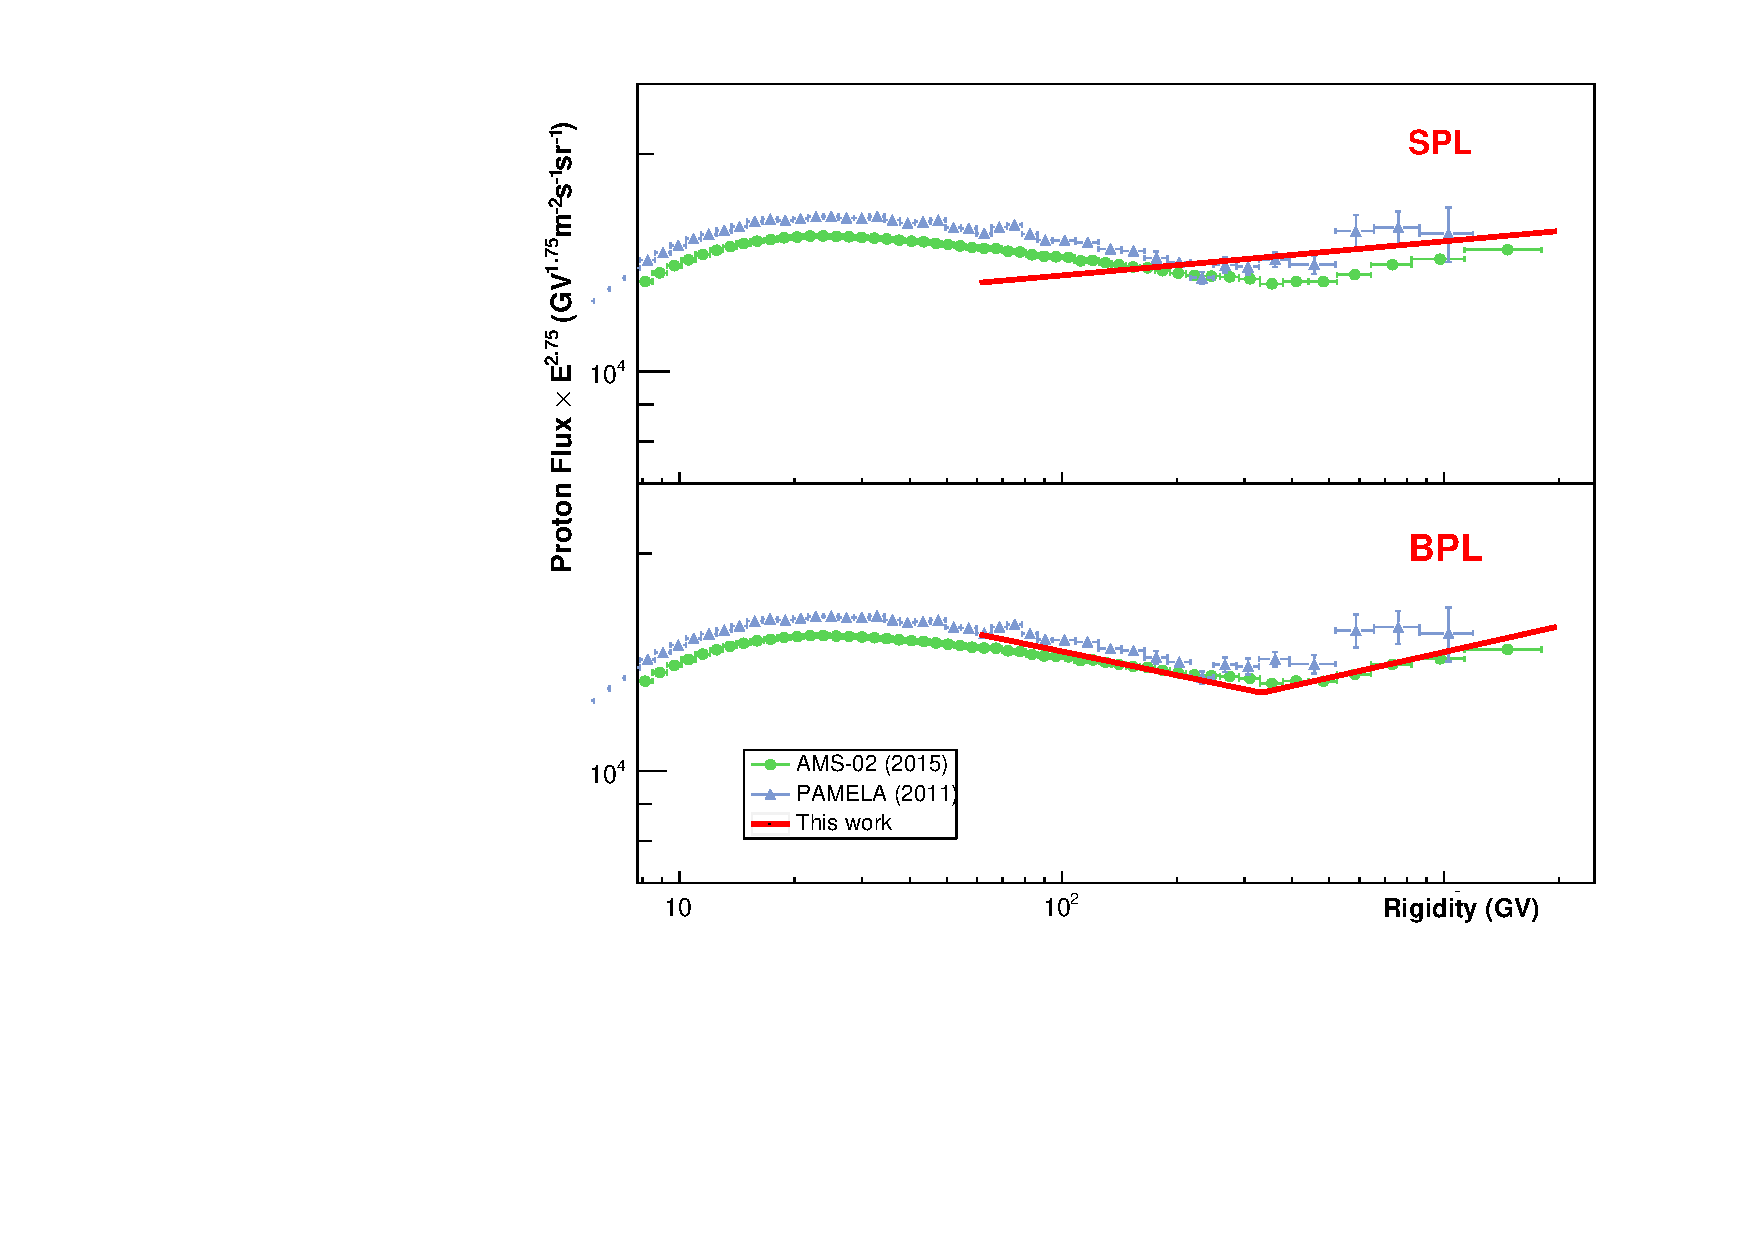
\includegraphics[width=0.8\textwidth]{img/ProtonSpectrumModelMeasurement.pdf}
    % \caption{Best fitted proton CRs versus real observations}
    \caption{Best-fit CR proton spectrum from this work (red) compared to the measurements by AMS-02 (blue) and PAMELA (green).}
    \label{fig:proton-flux}
\end{figure}



\section{Discussion and future work}
The best-fit BPL model of CR proton from this work are consistent with direct
measurements as shown in figure~\ref{fig:proton-flux}.
% The result also put weight on the previous study that we could take a
% benefit of brightness $\gamma$-ray from Earth's high atmosphere to indirectly observe cosmic
% ray spectrum which cause it’s luminosity.
We will need to determine whether the BPL model fits the data significantly better
than the SPL model does using likelihood ratio test to quantify the level of
confidence. We also plan to determine the statistical and total uncertainties of
the fit results by performing Monte Carlo simulations.
This work emphasizes that we could utilize the bright $\gamma$-ray emission
of the Earth's upper atmosphere to indirectly observe various properties of CRs.

\begin{figure}
    \centering
    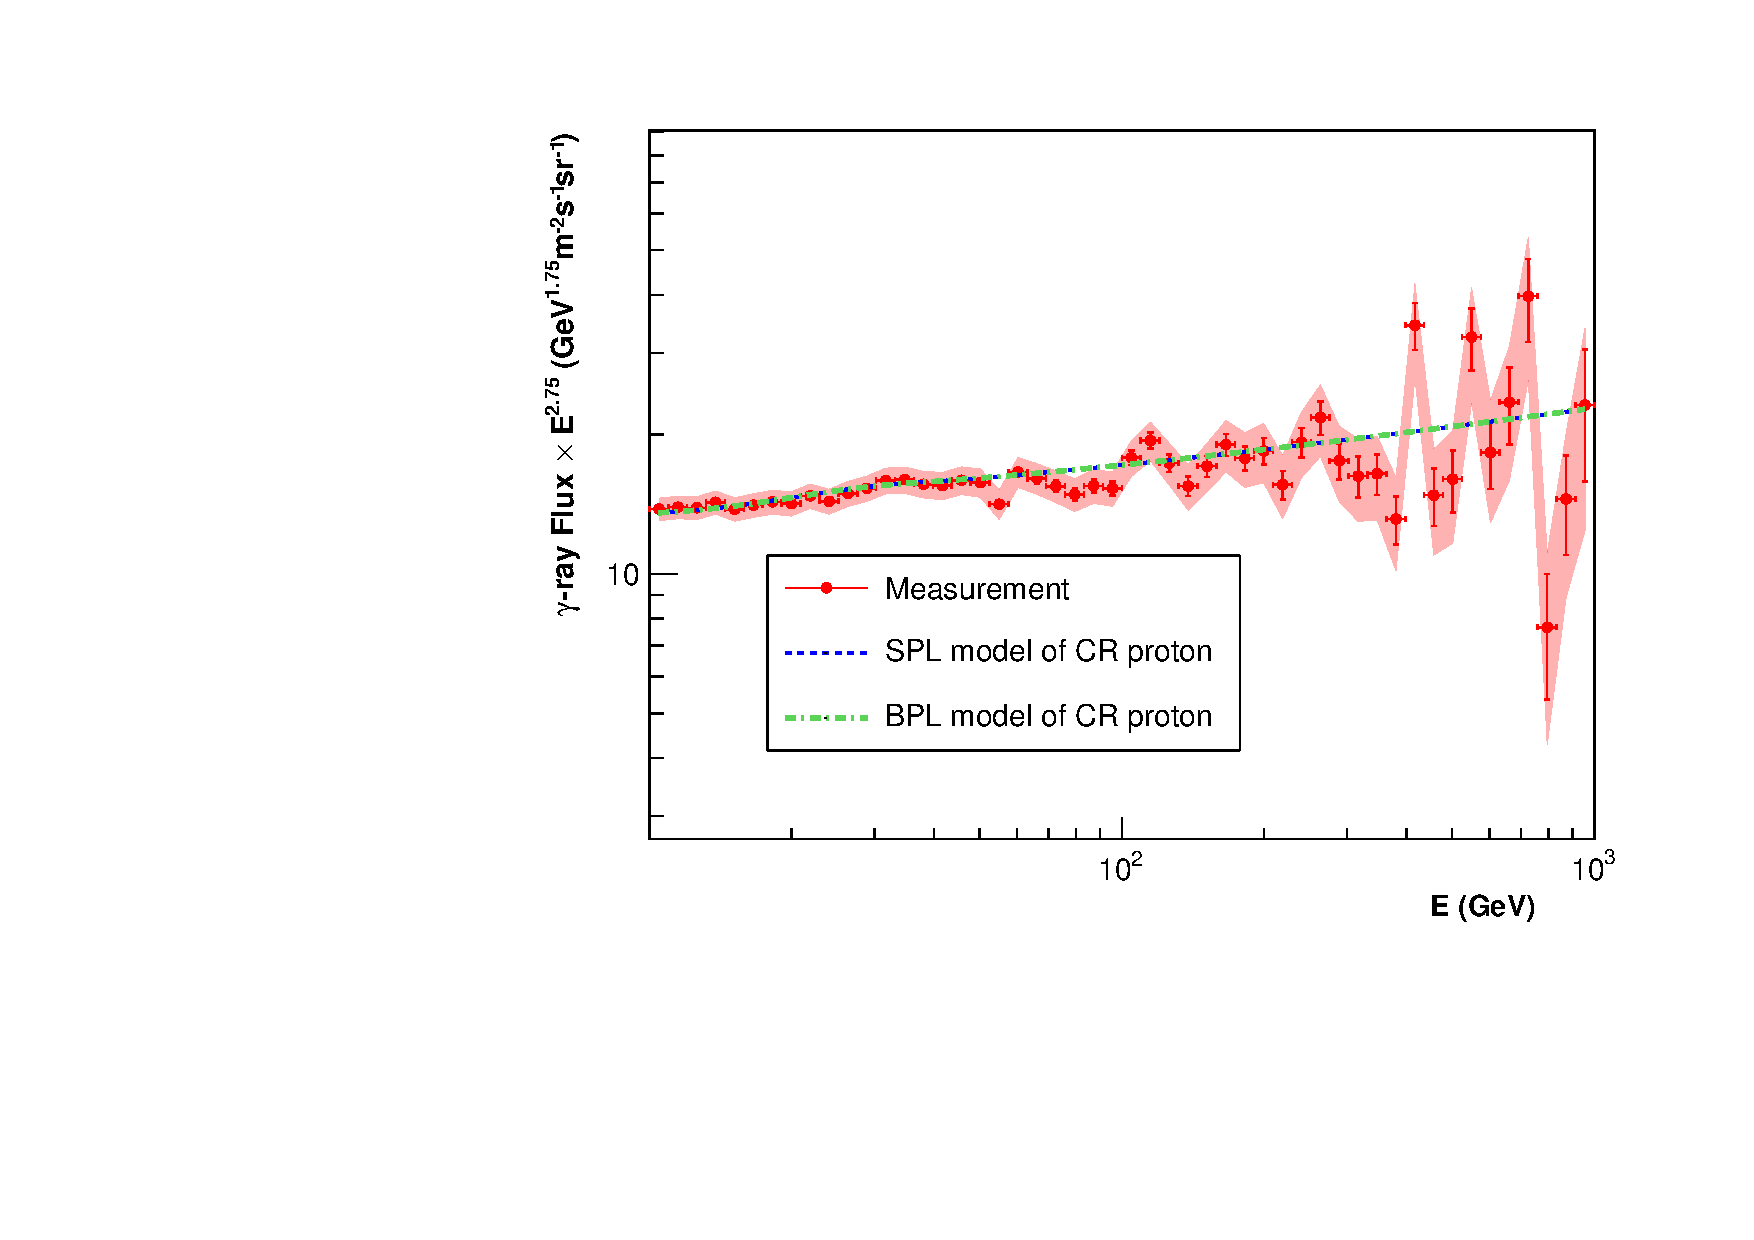
\includegraphics[width=0.8\textwidth]{img/fitted_result}
    % \caption{Measured $\gamma$-ray flux and the product from incident CRs}
    \caption{
        The $\gamma$-ray spectra calculated from the SPL (blue)
        and BPL (green) models of CR proton which best fit with the measured Earth's
        $\gamma$-ray spectrum in the thin-target regime (red).
    }
    \label{fig:gamma-flux}
\end{figure}


\begin{center}
\begin{table}
\centering
\caption{Best-fit CR proton spectral parameters.} 
\label{tb:bestparams}
\begin{tabular}{@{}l*{15}{l}}
\br
CR proton model&Index 1&Index 2&$E_\text{break}$ (GeV)\\
\mr
SPL&2.70&-&-\\
BPL&2.86&2.63&333\\
\br
\end{tabular}
\end{table}
\end{center}


\begin{figure}
    \centering
    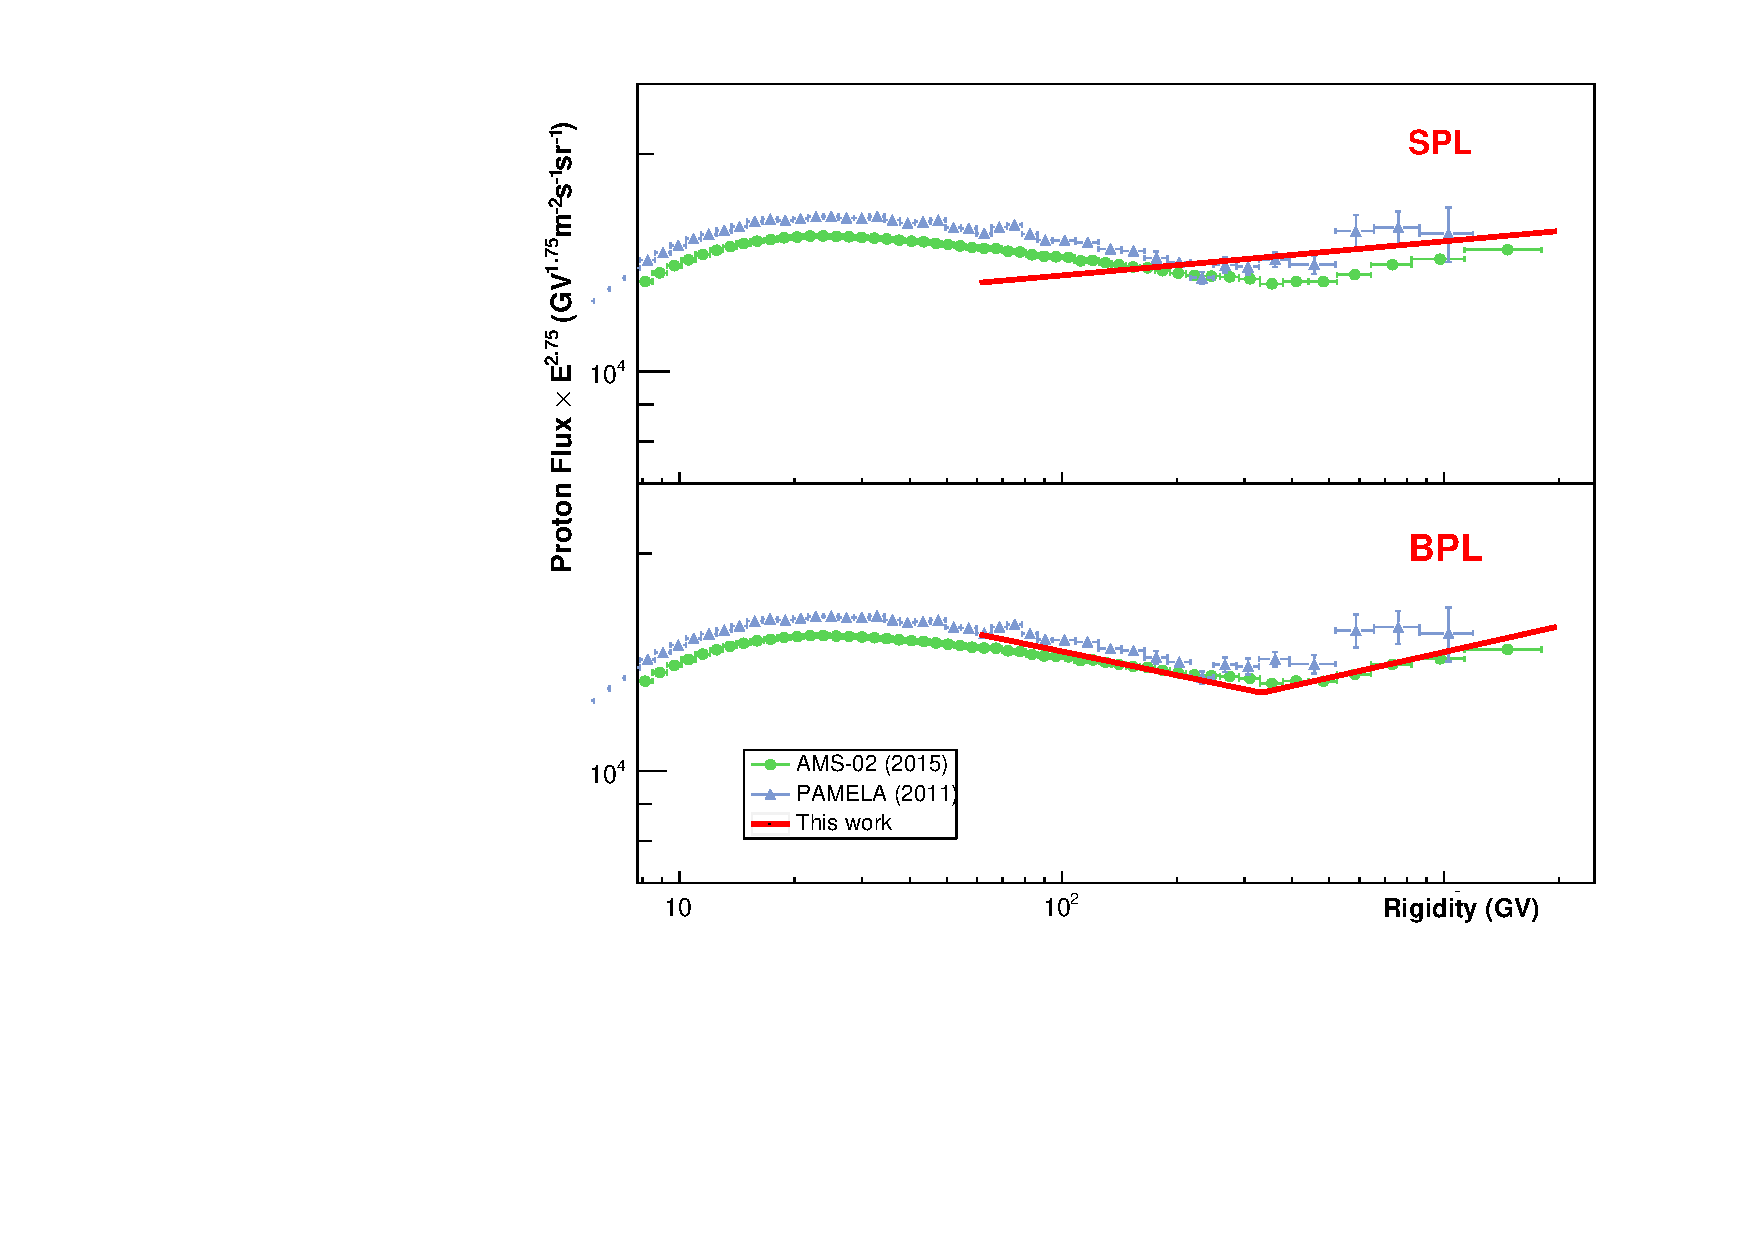
\includegraphics[width=0.9\textwidth]{img/ProtonSpectrumModelMeasurement.pdf}
    % \caption{Best fitted proton CRs versus real observations}
    \caption{Best-fit CR proton spectrum from this work (red) compared to the measurements by AMS-02 (blue) and PAMELA (green).}
    \label{fig:proton-flux}
\end{figure}

% From Figure~\ref{fig:gamma-flux}, a trend of incident proton model
% demonstrated that BPL has more consistency than SPL. Nevertheless,
% to determine the significance between two models require likelihood
% ratio test to evaluate the statistical level of confidence. In addition,
% statistical and total error including the instrument will be determined
% by performing Monte Carlo Simulation.







% after this is the example

% \section{Preparing your paper}
% \verb"jpconf" requires \LaTeXe\ and  can be used with other package files such
% as those loading the AMS extension fonts 
% \verb"msam" and \verb"msbm" (these fonts provide the 
% blackboard bold alphabet and various extra maths symbols as well as 
% symbols useful in figure captions); an extra style file \verb"iopams.sty" is 
% provided to load these packages and provide extra definitions for bold Greek letters. 
% \subsection{Headers, footers and page numbers}
% Authors should {\it not} add headers, footers or page numbers to the pages of their article---they will
% be added by \iopp\ as part of the production process.

% \subsection{{\cls\ }package options}
% The \cls\ class file has two options `a4paper' and `letterpaper':
% \begin{verbatim}
% \documentclass[a4paper]{jpconf}
% \end{verbatim}

% or \begin{verbatim}
% \documentclass[letterpaper]{jpconf}
% \end{verbatim}

% \begin{center}
% \begin{table}[h]
% \caption{\label{opt}\cls\ class file options.}
% %\footnotesize\rm
% \centering
% \begin{tabular}{@{}*{7}{l}}
% \br
% Option&Description\\
% \mr
% \verb"a4paper"&Set the paper size and margins for A4 paper.\\
% \verb"letterpaper"&Set the paper size and margins for US letter paper.\\
% \br
% \end{tabular}
% \end{table}
% \end{center}

% The default paper size is A4 (i.e., the default option is {\tt a4paper}) but this can be changed to Letter by 
% using \verb"\documentclass[letterpaper]{jpconf}". It is essential that you do not put macros into the text which alter the page dimensions.

% \section{The title, authors, addresses and abstract} 
% The code for setting the title page information is slightly different from
% the normal default in \LaTeX\ but please follow these instructions as carefully as possible so all articles within a conference have the same style to the title page. 
% The title is set in bold unjustified type using the command
% \verb"\title{#1}", where \verb"#1" is the title of the article. The
% first letter of the title should be capitalized with the rest in lower case. 
% The next information required is the list of all authors' names followed by 
% the affiliations. For the authors' names type \verb"\author{#1}", 
% where \verb"#1" is the 
% list of all authors' names. The style for the names is initials then
% surname, with a comma after all but the last 
% two names, which are separated by `and'. Initials should {\it not} have 
% full stops. First names may be used if desired. The command \verb"\maketitle" is not
% required.

% The addresses of the authors' affiliations follow the list of authors. 
% Each address should be set by using
% \verb"\address{#1}" with the address as the single parameter in braces. 
% If there is more 
% than one address then a superscripted number, followed by a space, should come at the start of
% each address. In this case each author should also have a superscripted number or numbers following their name to indicate which address is the appropriate one for them.
 
% Please also provide e-mail addresses for any or all of the authors using an \verb"\ead{#1}" command after the last address. \verb"\ead{#1}" provides the text Email: so \verb"#1" is just the e-mail address or a list of emails.  

% The abstract follows the addresses and
% should give readers concise information about the content 
% of the article and should not normally exceed 200 
% words. {\bf All articles must include an abstract}. To indicate the start 
% of the abstract type \verb"\begin{abstract}" followed by the text of the 
% abstract.  The abstract should normally be restricted 
% to a single paragraph and is terminated by the command
% \verb"\end{abstract}"

% \subsection{Sample coding for the start of an article}
% \label{startsample}
% The code for the start of a title page of a typical paper might read:
% \begin{verbatim}
% \title{The anomalous magnetic moment of the 
% neutrino and its relation to the solar neutrino problem}

% \author{P J Smith$^1$, T M Collins$^2$, 
% R J Jones$^{3,}$\footnote[4]{Present address:
% Department of Physics, University of Bristol, Tyndalls Park Road, 
% Bristol BS8 1TS, UK.} and Janet Williams$^3$}

% \address{$^1$ Mathematics Faculty, Open University, 
% Milton Keynes MK7~6AA, UK}
% \address{$^2$ Department of Mathematics, 
% Imperial College, Prince Consort Road, London SW7~2BZ, UK}
% \address{$^3$ Department of Computer Science, 
% University College London, Gower Street, London WC1E~6BT, UK}

% \ead{williams@ucl.ac.uk}

% \begin{abstract}
% The abstract appears here.
% \end{abstract}
% \end{verbatim}

% \section{The text}
% The text of the article should should be produced using standard \LaTeX\ formatting. Articles may be divided into sections and subsections, but the length limit provided by the \corg\ should be adhered to.

% \subsection{Acknowledgments}
% Authors wishing to acknowledge assistance or encouragement from 
% colleagues, special work by technical staff or financial support from 
% organizations should do so in an unnumbered Acknowledgments section 
% immediately following the last numbered section of the paper. The 
% command \verb"\ack" sets the acknowledgments heading as an unnumbered
% section.

% \subsection{Appendices}
% Technical detail that it is necessary to include, but that interrupts 
% the flow of the article, may be consigned to an appendix. 
% Any appendices should be included at the end of the main text of the paper, after the acknowledgments section (if any) but before the reference list.
% If there are two or more appendices they will be called Appendix A, Appendix B, etc. 
% Numbered equations will be in the form (A.1), (A.2), etc,
% figures will appear as figure A1, figure B1, etc and tables as table A1,
% table B1, etc.

% The command \verb"\appendix" is used to signify the start of the
% appendixes. Thereafter \verb"\section", \verb"\subsection", etc, will 
% give headings appropriate for an appendix. To obtain a simple heading of 
% `Appendix' use the code \verb"\section*{Appendix}". If it contains
% numbered equations, figures or tables the command \verb"\appendix" should
% precede it and \verb"\setcounter{section}{1}" must follow it. 

% \section{References}
% %%%%%%%%%%%%%%%%%%%%%%%%%%%%%%%%%%%%%%%%%%%
% In the online version of \jpcs\ references will be linked to their original source or to the article within a secondary service such as INSPEC or ChemPort wherever possible. To facilitate this linking extra care should be taken when preparing reference lists. 

% Two different styles of referencing are in common use: the Harvard alphabetical system and the Vancouver numerical system.  For \jpcs, the Vancouver numerical system is preferred but authors should use the Harvard alphabetical system if they wish to do so. In the numerical system references are numbered sequentially throughout the text within square brackets, like this [2], and one number can be used to designate several references.  

% \subsection{Using \BibTeX}
% We highly recommend the {\ttfamily\textbf\selectfont iopart-num} \BibTeX\ package by Mark~A~Caprio \cite{HESS}, which is included with this documentation.

% \subsection{Reference lists}
% A complete reference should provide the reader with enough information to locate the article concerned, whether published in print or electronic form, and should, depending on the type of reference, consist of:  

% \begin{itemize}
% \item name(s) and initials;
% \item date published;
% \item title of journal, book or other publication; 
% \item titles of journal articles may also be included (optional);
% \item volume number;
% \item editors, if any;
% \item town of publication and publisher in parentheses for {\it books};
% \item the page numbers.
% \end{itemize}

% Up to ten authors may be given in a particular reference; where 
% there are more than ten only the first should be given followed by 
% `{\it et al}'. If an author is unsure of a particular journal's abbreviated title it is best to leave the title in 
% full. The terms {\it loc.\ cit.\ }and {\it ibid.\ }should not be used. 
% Unpublished conferences and reports should generally not be included 
% in the reference list and articles in the course of publication should 
% be entered only if the journal of publication is known. 
% A thesis submitted for a higher degree may be included 
% in the reference list if it has not been superseded by a published 
% paper and is available through a library; sufficient information 
% should be given for it to be traced readily.

% \subsection{Formatting reference lists}
% Numeric reference lists should contain the references within an unnumbered section (such as \verb"\section*{References}"). The 
% reference list itself is started by the code 
% \verb"\begin{thebibliography}{<num>}", where \verb"<num>" is the largest
% number in the reference list and is completed by
% \verb"\end{thebibliography}". 
% Each reference starts with \verb"\bibitem{<label>}", where `label' is the label used for cross-referencing. Each \verb"\bibitem" should only contain a reference to a single article (or a single article and a preprint reference to the same article).  When one number actually covers a group of two or more references to different articles, \verb"\nonum"
% should replace \verb"\bibitem{<label>}" at
% the start of each reference in the group after the first.

% For an alphabetic reference list use \verb"\begin{thereferences}" ... \verb"\end{thereferences}" instead of the
% `thebibliography' environment and each reference can be start with just \verb"\item" instead of \verb"\bibitem{label}"
% as cross referencing is less useful for alphabetic references.

% \subsection {References to printed journal articles}
% A normal reference to a journal article contains three changes of font (see table \ref{jfonts}) and is constructed as follows:

% \begin{itemize}
% \item the authors should be in the form surname (with only the first letter capitalized) followed by the initials with no periods after the initials. Authors should be separated by a comma except for the last two which should be separated by `and' with no comma preceding it;
% \item the article title (if given) should be in lower case letters, except for an initial capital, and should follow the date;
% \item the journal title is in italic and is abbreviated. If a journal has several parts denoted by different letters the part letter should be inserted after the journal in Roman type, e.g. {\it Phys. Rev.} A;
% \item the volume number should be in bold type;
% \item both the initial and final page numbers should be given where possible. The final page number should be in the shortest possible form and separated from the initial page number by an en rule `-- ', e.g. 1203--14, i.e. the numbers `12' are not repeated.
% \end{itemize}

% A typical (numerical) reference list might begin

% \medskip
% \begin{thebibliography}{9}
% \item Strite S and Morkoc H 1992 {\it J. Vac. Sci. Technol.} B {\bf 10} 1237 
% \item Jain S C, Willander M, Narayan J and van Overstraeten R 2000 
% {\it J. Appl. Phys}. {\bf 87} 965 
% \item Nakamura S, Senoh M, Nagahama S, Iwase N, Yamada T, Matsushita T, Kiyoku H 
% and 	Sugimoto Y 1996 {\it Japan. J. Appl. Phys.} {\bf 35} L74 
% \item Akasaki I, Sota S, Sakai H, Tanaka T, Koike M and Amano H 1996 
% {\it Electron. Lett.} {\bf 32} 1105 
% \item O'Leary S K, Foutz B E, Shur M S, Bhapkar U V and Eastman L F 1998 
% {\it J. Appl. Phys.} {\bf 83} 826 
% \item Jenkins D W and Dow J D 1989 {\it Phys. Rev.} B {\bf 39} 3317 
% \end{thebibliography}
% \smallskip

% \noindent which would be obtained by typing

% \begin{verbatim}
% \begin{\thebibliography}{9}
% \item Strite S and Morkoc H 1992 {\it J. Vac. Sci. Technol.} B {\bf 10} 1237 
% \item Jain S C, Willander M, Narayan J and van Overstraeten R 2000 
% {\it J. Appl. Phys}. {\bf 87} 965 
% \item Nakamura S, Senoh M, Nagahama S, Iwase N, Yamada T, Matsushita T, Kiyoku H 
% and 	Sugimoto Y 1996 {\it Japan. J. Appl. Phys.} {\bf 35} L74 
% \item Akasaki I, Sota S, Sakai H, Tanaka T, Koike M and Amano H 1996 
% {\it Electron. Lett.} {\bf 32} 1105 
% \item O'Leary S K, Foutz B E, Shur M S, Bhapkar U V and Eastman L F 1998 
% {\it J. Appl. Phys.} {\bf 83} 826 
% \item Jenkins D W and Dow J D 1989 {\it Phys. Rev.} B {\bf 39} 3317 
% \end{\thebibliography}
% \end{verbatim}

% \begin{center}
% \begin{table}[h]
% \centering
% \caption{\label{jfonts}Font styles for a reference to a journal article.} 
% \begin{tabular}{@{}l*{15}{l}}
% \br
% Element&Style\\
% \mr
% Authors&Roman type\\
% Date&Roman type\\
% Article title (optional)&Roman type\\
% Journal title&Italic type\\
% Volume number&Bold type\\
% Page numbers&Roman type\\
% \br
% \end{tabular}
% \end{table}
% \end{center}

% \subsection{References to \jpcs\ articles}
% Each conference proceeding published in \jpcs\ will be a separate {\it volume}; 
% references should follow the style for conventional printed journals. For example:\vspace{6pt}
% \numrefs{1}
% \item Douglas G 2004 \textit{J. Phys.: Conf. Series} \textbf{1} 23--36
% \endnumrefs

% %%%%%%%%%%%%%%%%%%%%%%%%%%%%%%%%%%
% \subsection{References to preprints}
% For preprints there are two distinct cases:
% \renewcommand{\theenumi}{\arabic{enumi}}
% \begin{enumerate}
% \item Where the article has been published in a journal and the preprint is supplementary reference information. In this case it should be presented as:
% \medskip
% \numrefs{1}
% \item Kunze K 2003 T-duality and Penrose limits of spatially homogeneous and inhomogeneous cosmologies {\it Phys. Rev.} D {\bf 68} 063517 ({\it Preprint} gr-qc/0303038)
% \endnumrefs
% \item Where the only reference available is the preprint. In this case it should be presented as
% \medskip
% \numrefs{1}
% \item Milson R, Coley A, Pravda V and Pravdova A 2004 Alignment and algebraically special tensors {\it Preprint} gr-qc/0401010
% \endnumrefs
% \end{enumerate}

% \subsection{References to electronic-only journals}
% In general article numbers are given, and no page ranges, as most electronic-only journals start each article on page 1.

% \begin{itemize} 
% \item For {\it New Journal of Physics} (article number may have from one to three digits)
% \numrefs{1}
% \item Fischer R 2004 Bayesian group analysis of plasma-enhanced chemical vapour deposition data {\it New. J. Phys.} {\bf 6} 25 
% \endnumrefs
% \item For SISSA journals the volume is divided into monthly issues and these form part of the article number

% \numrefs{2}
% \item Horowitz G T and Maldacena J 2004 The black hole final state {\it J. High Energy Phys.}  	JHEP02(2004)008
% \item Bentivegna E, Bonanno A and Reuter M 2004 Confronting the IR fixed point cosmology 	with 	high-redshift observations {\it J. Cosmol. Astropart. Phys.} JCAP01(2004)001  
% \endnumrefs
% \end{itemize} 

% \subsection{References to books, conference proceedings and reports}
% References to books, proceedings and reports are similar to journal references, but have 
% only two changes of font (see table~\ref{book}). 

% \begin{table}
% \centering
% \caption{\label{book}Font styles for references to books, conference proceedings and reports.}
% \begin{tabular}{@{}l*{15}{l}}
% \br
% Element&Style\\
% \mr
% Authors&Roman type\\
% Date&Roman type\\
% Book title (optional)&Italic type\\
% Editors&Roman type\\
% Place (city, town etc) of publication&Roman type\\
% Publisher&Roman type\\
% Volume&Roman type\\
% Page numbers&Roman type\\
% \br
% \end{tabular}
% \end{table}

% Points to note are:
% \medskip
% \begin{itemize}
% \item Book titles are in italic and should be spelt out in full with initial capital letters for all except minor words. Words such as Proceedings, Symposium, International, Conference, Second, etc should be abbreviated to {\it Proc.}, {\it Symp.}, {\it Int.}, {\it Conf.}, {\it 2nd}, respectively, but the rest of the title should be given in full, followed by the date of the conference and the town or city where the conference was held. For Laboratory Reports the Laboratory should be spelt out wherever possible, e.g. {\it Argonne National Laboratory Report}.
% \item The volume number, for example vol 2, should be followed by the editors, if any, in a form such as `ed A J Smith and P R Jones'. Use {\it et al} if there are more than two editors. Next comes the town of publication and publisher, within brackets and separated by a colon, and finally the page numbers preceded by p if only one number is given or pp if both the initial and final numbers are given.
% \end{itemize}

% Examples taken from published papers:
% \medskip

% \numrefs{99}
% \item Kurata M 1982 {\it Numerical Analysis for Semiconductor Devices} (Lexington, MA: Heath)
% \item Selberherr S 1984 {\it Analysis and Simulation of Semiconductor Devices} (Berlin: Springer)
% \item Sze S M 1969 {\it Physics of Semiconductor Devices} (New York: Wiley-Interscience)
% \item Dorman L I 1975 {\it Variations of Galactic Cosmic Rays} (Moscow: Moscow State University Press) p 103
% \item Caplar R and Kulisic P 1973 {\it Proc. Int. Conf. on Nuclear Physics (Munich)} vol 1 (Amsterdam: 	North-Holland/American Elsevier) p 517
% \item Cheng G X 2001 {\it Raman and Brillouin Scattering-Principles and Applications} (Beijing: Scientific) 
% \item Szytula A and Leciejewicz J 1989 {\it Handbook on the Physics and Chemistry of Rare Earths} vol 12, ed K A Gschneidner Jr and L Erwin (Amsterdam: Elsevier) p 133
% \item Kuhn T 1998 {\it Density matrix theory of coherent ultrafast dynamics Theory of Transport Properties of Semiconductor Nanostructures} (Electronic Materials vol 4) ed E Sch\"oll (London: Chapman and Hall) chapter 6 pp 173--214
% \endnumrefs

% \section{Tables and table captions}
% Tables should be numbered serially and referred to in the text 
% by number (table 1, etc, {\bf rather than} tab. 1). Each table should be a float and be positioned within the text at the most convenient place near to where it is first mentioned in the text. It should have an 
% explanatory caption which should be as concise as possible. 

% \subsection{The basic table format}
% The standard form for a table is:
% \begin{verbatim}
% \begin{table}
% \caption{\label{label}Table caption.}
% \begin{center}
% \begin{tabular}{llll}
% \br
% Head 1&Head 2&Head 3&Head 4\\
% \mr
% 1.1&1.2&1.3&1.4\\
% 2.1&2.2&2.3&2.4\\
% \br
% \end{tabular}
% \end{center}
% \end{table}
% \end{verbatim}

% The above code produces table~\ref{ex}.

% \begin{table}[h]
% \caption{\label{ex}Table caption.}
% \begin{center}
% \begin{tabular}{llll}
% \br
% Head 1&Head 2&Head 3&Head 4\\
% \mr
% 1.1&1.2&1.3&1.4\\
% 2.1&2.2&2.3&2.4\\
% \br
% \end{tabular}
% \end{center}
% \end{table}

% Points to note are:
% \medskip
% \begin{enumerate}
% \item The caption comes before the table.
% \item The normal style is for tables to be centred in the same way as
% equations. This is accomplished
% by using \verb"\begin{center}" \dots\ \verb"\end{center}".

% \item The default alignment of columns should be aligned left.

% \item Tables should have only horizontal rules and no vertical ones. The rules at
% the top and bottom are thicker than internal rules and are set with
% \verb"\br" (bold rule). 
% The rule separating the headings from the entries is set with
% \verb"\mr" (medium rule). These commands do not need a following double backslash.

% \item Numbers in columns should be aligned as appropriate, usually on the decimal point;
% to help do this a control sequence \verb"\lineup" has been defined 
% which sets \verb"\0" equal to a space the size of a digit, \verb"\m"
% to be a space the width of a minus sign, and \verb"\-" to be a left
% overlapping minus sign. \verb"\-" is for use in text mode while the other
% two commands may be used in maths or text.
% (\verb"\lineup" should only be used within a table
% environment after the caption so that \verb"\-" has its normal meaning
% elsewhere.) See table~\ref{tabone} for an example of a table where
% \verb"\lineup" has been used.
% \end{enumerate}

% \begin{table}[h]
% \caption{\label{tabone}A simple example produced using the standard table commands 
% and $\backslash${\tt lineup} to assist in aligning columns on the 
% decimal point. The width of the 
% table and rules is set automatically by the 
% preamble.} 

% \begin{center}
% \lineup
% \begin{tabular}{*{7}{l}}
% \br                              
% $\0\0A$&$B$&$C$&\m$D$&\m$E$&$F$&$\0G$\cr 
% \mr
% \0\023.5&60  &0.53&$-20.2$&$-0.22$ &\01.7&\014.5\cr
% \0\039.7&\-60&0.74&$-51.9$&$-0.208$&47.2 &146\cr 
% \0123.7 &\00 &0.75&$-57.2$&\m---   &---  &---\cr 
% 3241.56 &60  &0.60&$-48.1$&$-0.29$ &41   &\015\cr 
% \br
% \end{tabular}
% \end{center}
% \end{table}
 
% \section{Figures and figure captions}
% Figures must be included in the source code of an article at the appropriate place in the text not grouped together at the end. 

% Each figure should have a brief caption describing it and, if 
% necessary, interpreting the various lines and symbols on the figure. 
% As much lettering as possible should be removed from the figure itself and 
% included in the caption. If a figure has parts, these should be 
% labelled ($a$), ($b$), ($c$), etc. 
% \Tref{blobs} gives the definitions for describing symbols and lines often
% used within figure captions (more symbols are available
% when using the optional packages loading the AMS extension fonts).

% \begin{table}[h]
% \caption{\label{blobs}Control sequences to describe lines and symbols in figure 
% captions.}
% \begin{center}
% \begin{tabular}{lllll}
% \br
% Control sequence&Output&&Control sequence&Output\\
% \mr
% \verb"\dotted"&\dotted        &&\verb"\opencircle"&\opencircle\\
% \verb"\dashed"&\dashed        &&\verb"\opentriangle"&\opentriangle\\
% \verb"\broken"&\broken&&\verb"\opentriangledown"&\opentriangledown\\
% \verb"\longbroken"&\longbroken&&\verb"\fullsquare"&\fullsquare\\
% \verb"\chain"&\chain          &&\verb"\opensquare"&\opensquare\\
% \verb"\dashddot"&\dashddot    &&\verb"\fullcircle"&\fullcircle\\
% \verb"\full"&\full            &&\verb"\opendiamond"&\opendiamond\\
% \br
% \end{tabular}
% \end{center}
% \end{table}


% Authors should try and use the space allocated to them as economically as possible. At times it may be convenient to put two figures side by side or the caption at the side of a figure. To put figures side by side, within a figure environment, put each figure and its caption into a minipage with an appropriate width (e.g. 3in or 18pc if the figures are of equal size) and then separate the figures slightly by adding some horizontal space between the two minipages (e.g. \verb"\hspace{.2in}" or \verb"\hspace{1.5pc}". To get the caption at the side of the figure add the small horizontal space after the \verb"\includegraphics" command and then put the \verb"\caption" within a minipage of the appropriate width aligned bottom, i.e. \verb"\begin{minipage}[b]{3in}" etc (see code in this file used to generate figures 1--3).

% Note that it may be necessary to adjust the size of the figures (using optional arguments to \verb"\includegraphics", for instance \verb"[width=3in]") to get you article to fit within your page allowance or to obtain good page breaks.

% \begin{figure}[h]
% \begin{minipage}{14pc}
% 
\includegraphics[width=14pc]{name.eps}
% \caption{\label{label}Figure caption for first of two sided figures.}
% \end{minipage}\hspace{2pc}%
% \begin{minipage}{14pc}
% 
\includegraphics[width=14pc]{name.eps}
% \caption{\label{label}Figure caption for second of two sided figures.}
% \end{minipage} 
% \end{figure}

% \begin{figure}[h]
% 
\includegraphics[width=14pc]{name.eps}\hspace{2pc}%
% \begin{minipage}[b]{14pc}\caption{\label{label}Figure caption for a narrow figure where the caption is put at the side of the figure.}
% \end{minipage}
% \end{figure}

% Using the graphicx package figures can be included using code such as:
% \begin{verbatim}
% \begin{figure}
% \begin{center}
% \includegraphics{file.eps}
% \end{center}
% \caption{\label{label}Figure caption}
% \end{figure}
% \end{verbatim}


\section*{References}
% \bibliographystyle{abbrv}
\bibliographystyle{iopart-num}
% \bibliographystyle{unsrt}
\bibliography{iopart-num_short}

\end{document}


